\documentclass{article}
% translate with >> pdflatex -shell-escape <file>

% This file is used as unit test for pgfplots, copyright by Christian Feuersaenger.
% 
% See
%   http://pgfplots.sourceforge.net/pgfplots.pdf
% for pgfplots.
%
% Any required input files (for <plot table> or <plot file> or the table package) can be downloaded
% at
% http://www.ctan.org/tex-archive/graphics/pgf/contrib/pgfplots/doc/latex/
% and
% http://www.ctan.org/tex-archive/graphics/pgf/contrib/pgfplots/doc/latex/plotdata/

\usepackage{pgfplots}
\pgfplotsset{compat=newest}

\pagestyle{empty}


\begin{document}

	\newcommand\TESTS{
		\subsubsection{tick pos=both}
		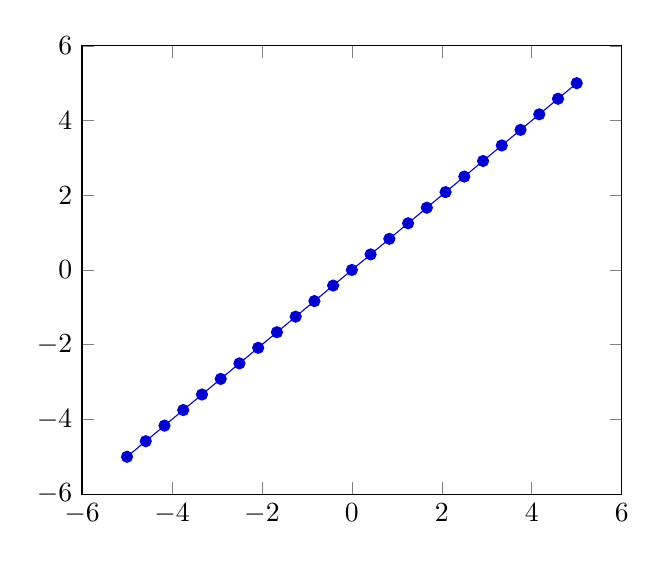
\begin{tikzpicture}
			\begin{axis}[
				tick pos=both,
			]

			\addplot {x};
			\end{axis}
		\end{tikzpicture}

		\subsubsection{tick pos=left}
		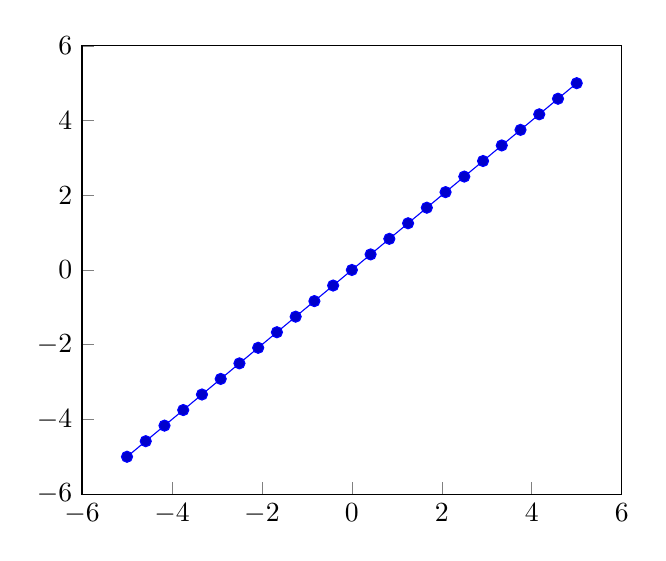
\begin{tikzpicture}
			\begin{axis}[
				tick pos=left,
			]

			\addplot {x};
			\end{axis}
		\end{tikzpicture}

		\subsubsection{tick pos=right}
		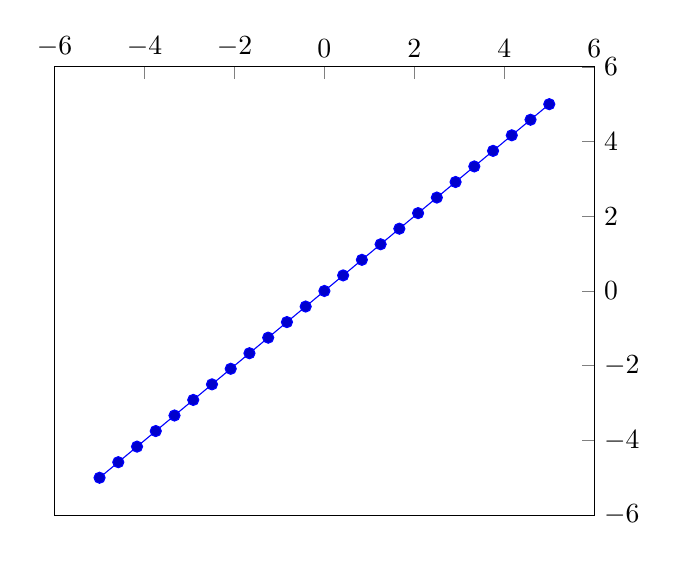
\begin{tikzpicture}
			\begin{axis}[
				tick pos=right,
			]

			\addplot {x};
			\end{axis}
		\end{tikzpicture}


		\subsubsection{ticklabel pos=left}
		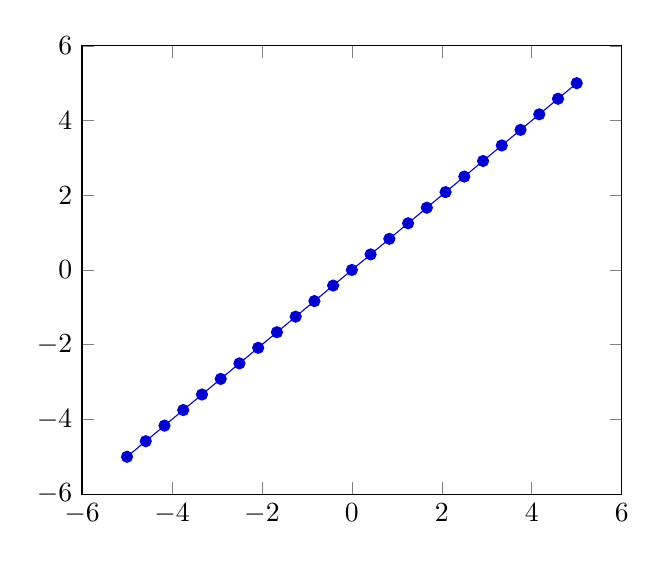
\begin{tikzpicture}
			\begin{axis}[
				ticklabel pos=left,
			]

			\addplot {x};
			\end{axis}
		\end{tikzpicture}

		\subsubsection{ticklabel pos=right}
		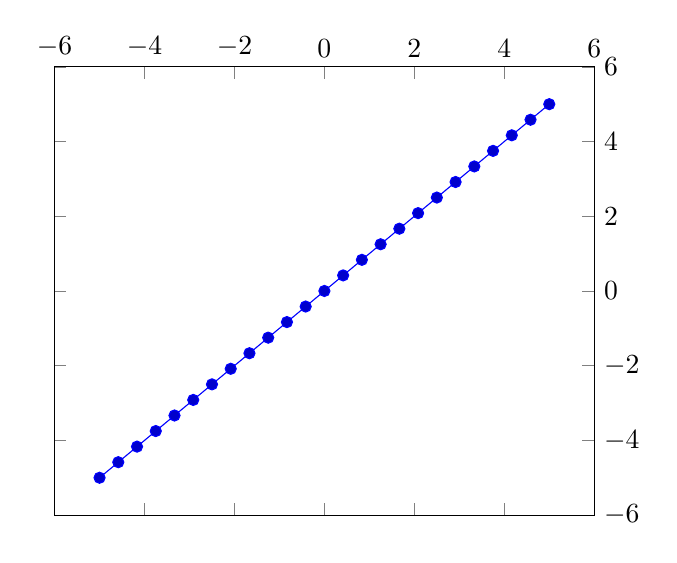
\begin{tikzpicture}
			\begin{axis}[
				ticklabel pos=right,
			]

			\addplot {x};
			\end{axis}
		\end{tikzpicture}
	}

	\subsection{Standard}
	\TESTS

	\subsection{Reversed axes}
	{
		\pgfplotsset{x dir=reverse,y dir=reverse}
		\TESTS
	}
	\subsection{axis lines =center}
	{
		\pgfplotsset{axis lines=center}
		\TESTS
	}
	\subsection{axis lines =left}
	{
		\pgfplotsset{axis lines=left}
		\TESTS
	}
	\subsection{axis lines =right}
	{
		\pgfplotsset{axis lines=right}
		\TESTS
	}

	{
		\pgfplotsset{x dir=reverse,y dir=reverse}
		\subsection{reversed axes and axis lines =center}
		{
			\pgfplotsset{axis lines=center}
			\TESTS
		}
		\subsection{reversed axes and axis lines =left}
		{
			\pgfplotsset{axis lines=left}
			\TESTS
		}
		\subsection{reversed axes and axis lines =right}
		{
			\pgfplotsset{axis lines=right}
			\TESTS
		}
	}
\end{document}
